\documentclass[11pt]{article}
\usepackage[latin1]{inputenc}
\usepackage{a4wide}
\usepackage{amsmath}
\usepackage{amsfonts}
\usepackage{amssymb}
\usepackage{graphicx}
\usepackage{enumerate}
\usepackage{epstopdf}
\usepackage{float}
\usepackage{multicol}
\usepackage{hyperref}
\epstopdfsetup{outdir=./images/}

\title{Natural Computing, Assignment 2}
\author{Pauline Lauron - s1016609 \and Dennis Verheijden - s4455770 \and Joost Besseling - s4796799}
\begin{document}
\maketitle

\section{Using the Negative Selection Algorithm}
\begin{enumerate}[1.]
\item The ROC curve for the parameters $n=10, r=4$ may be observed in figure \ref{fig:ROC_ex1} as the orange line. The corresponding AUC is 0.7835, which is actually pretty good. The algorithm definitely learned whether the language is English or not.
\item The ROC curves for the parameters $r=1$ and $r=9$ are shown in figure \ref{fig:ROC_ex1} as respectively the green and blue line. Changing the length of the substrings ($r$), we can see some interesting results. If the length is 9, the ROC curve is basically chance. If the length is 1, the TPR and FPR values are almost constant since it just cannot distinguish anything.
\item \textbf{TODO:} Which language can be discriminated best?
\end{enumerate}

\begin{figure}[H]
\centering
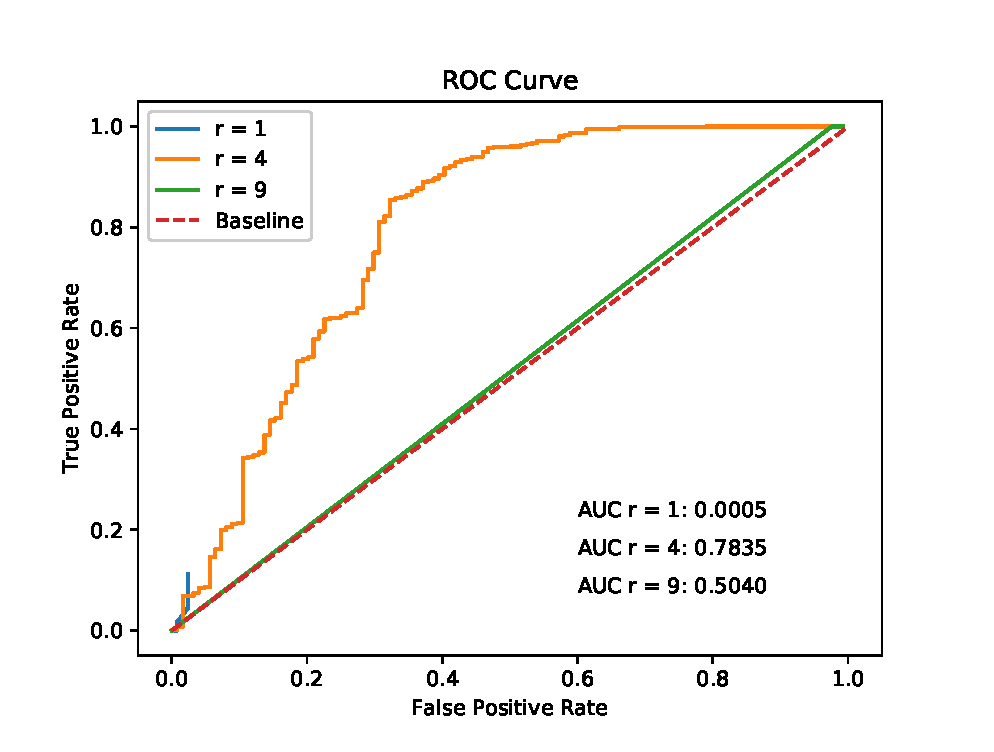
\includegraphics[width=0.7\textwidth]{images/roc_ex1.eps}
\caption{ROC curve for different values of $r$ in the negative selection algorithm}
\label{fig:ROC_ex1}
\end{figure}

\section{Intrusion Detection for Unix Processes}
\begin{itemize}
\item Detect anomalous sequences in the system calls datasets.
\item Do AUC analysis
\end{itemize}

\end{document}